\documentclass[a4paper, titlepage, 12pt]{article}\usepackage[]{graphicx}\usepackage[]{color}
%% maxwidth is the original width if it is less than linewidth
%% otherwise use linewidth (to make sure the graphics do not exceed the margin)
\makeatletter
\def\maxwidth{ %
  \ifdim\Gin@nat@width>\linewidth
    \linewidth
  \else
    \Gin@nat@width
  \fi
}
\makeatother

\definecolor{fgcolor}{rgb}{0.345, 0.345, 0.345}
\newcommand{\hlnum}[1]{\textcolor[rgb]{0.686,0.059,0.569}{#1}}%
\newcommand{\hlstr}[1]{\textcolor[rgb]{0.192,0.494,0.8}{#1}}%
\newcommand{\hlcom}[1]{\textcolor[rgb]{0.678,0.584,0.686}{\textit{#1}}}%
\newcommand{\hlopt}[1]{\textcolor[rgb]{0,0,0}{#1}}%
\newcommand{\hlstd}[1]{\textcolor[rgb]{0.345,0.345,0.345}{#1}}%
\newcommand{\hlkwa}[1]{\textcolor[rgb]{0.161,0.373,0.58}{\textbf{#1}}}%
\newcommand{\hlkwb}[1]{\textcolor[rgb]{0.69,0.353,0.396}{#1}}%
\newcommand{\hlkwc}[1]{\textcolor[rgb]{0.333,0.667,0.333}{#1}}%
\newcommand{\hlkwd}[1]{\textcolor[rgb]{0.737,0.353,0.396}{\textbf{#1}}}%

\usepackage{framed}
\makeatletter
\newenvironment{kframe}{%
 \def\at@end@of@kframe{}%
 \ifinner\ifhmode%
  \def\at@end@of@kframe{\end{minipage}}%
  \begin{minipage}{\columnwidth}%
 \fi\fi%
 \def\FrameCommand##1{\hskip\@totalleftmargin \hskip-\fboxsep
 \colorbox{shadecolor}{##1}\hskip-\fboxsep
     % There is no \\@totalrightmargin, so:
     \hskip-\linewidth \hskip-\@totalleftmargin \hskip\columnwidth}%
 \MakeFramed {\advance\hsize-\width
   \@totalleftmargin\z@ \linewidth\hsize
   \@setminipage}}%
 {\par\unskip\endMakeFramed%
 \at@end@of@kframe}
\makeatother

\definecolor{shadecolor}{rgb}{.97, .97, .97}
\definecolor{messagecolor}{rgb}{0, 0, 0}
\definecolor{warningcolor}{rgb}{1, 0, 1}
\definecolor{errorcolor}{rgb}{1, 0, 0}
\newenvironment{knitrout}{}{} % an empty environment to be redefined in TeX

\usepackage{alltt}
%\documentclass[nohyper,justified]{tufte-handout}

\usepackage[utf8x]{inputenc}
\usepackage{graphicx}
\usepackage{rotating}
\usepackage{mathptmx}      % use Times fonts if available on your TeX system
\usepackage{amsmath}
\usepackage{siunitx}
\usepackage{paralist}
\usepackage{mathtools}
\usepackage{amsfonts}
\usepackage{amssymb}
\usepackage{siunitx}
\usepackage{paralist}
\usepackage{ulem}
\usepackage[round]{natbib}

\usepackage{booktabs}
\usepackage{dcolumn}

\usepackage[titletoc, title]{appendix}
\newcommand{\HRule}{\rule{\linewidth}{3.0mm}}

% insert here the call for the packages your document requires
\usepackage{latexsym}
\usepackage{url}
\usepackage{hyperref}

\definecolor{brown}{rgb}{0.59, 0.29, 0.0}

\hypersetup{
  colorlinks   = true, %Colours links instead of ugly boxes
  urlcolor     = blue, %Colour for external hyperlinks
  linkcolor    = blue, %Colour of internal links
  citecolor    = black %Colour of citations
}

%**********************************************************************
% redefine thebibliography environment

\makeatletter
\renewenvironment{thebibliography}[1]
     {\section{\bibname}% <-- this line was changed from \chapter* to \section*
      \@mkboth{\MakeUppercase\bibname}{\MakeUppercase\bibname}%
      \list{\@biblabel{\@arabic\c@enumiv}}%
           {\settowidth\labelwidth{\@biblabel{#1}}%
            \leftmargin\labelwidth
            \advance\leftmargin\labelsep
            \@openbib@code
            \usecounter{enumiv}%
            \let\p@enumiv\@empty
            \renewcommand\theenumiv{\@arabic\c@enumiv}}%
      \sloppy
      \clubpenalty4000
      \@clubpenalty \clubpenalty
      \widowpenalty4000%
      \sfcode`\.\@m}
     {\def\@noitemerr
       {\@latex@warning{Empty `thebibliography' environment}}%
      \endlist}
\makeatother

%***********************************************************************
\IfFileExists{upquote.sty}{\usepackage{upquote}}{}
\begin{document}
\begin{sffamily}

\bibliographystyle{agsm}

\begin{titlepage}
\begin{center}

% Title\
\color{blue}
\HRule \\ [0.5cm]
\color{black}
{ \huge \bfseries Estimation\\of\\Irrigation Accession Volumes\\for\\the Berri, Cobdogla, Renmark and Chaffey Irrigation Districts\\ [0.5cm]}
\color{green}
\HRule \\ [3.0cm]
\color{black}

% Author and supervisor
\begin{center} \Large
\textbf{Tony \textsc{Meissner}} \\ [0.5cm]
{\large \textbf{\today}}
\end{center}

\color{white}
\HRule \\ [2.0cm]
\color{blue}
\begin{flushright}
\framebox[6.0cm]{
\colorbox{yellow}{
\begin{minipage}{0.35\textwidth}
\begin{flushleft}
\small
  Laroona Environmetrics \\
  PO Box 1102 \\
  Loxton SA 5333 Australia \\
  Tel.: +61 8 8587 6248 \\
  email: laroona.env01@bigpond.com
\end{flushleft}
\end{minipage}}
}
\end{flushright}
\color{brown}
\HRule \\
\color{black}
\end{center}
\end{titlepage}



\section{Introduction}
The Department for Environment, Water and Natural Resources (DEWNR) contracted Laroona Environmetrics to review accessions\footnote{\footnotesize{\bfseries{Accessions} are defined as the volume of water draining beyond the rootzone of irrigated crops that eventually percolates to the groundwater. Accessions volumes are not necessarily equal to groundwater recharge volumes. The presence of aquitards, lateral spread of the accession front and water held in the geological layers above the aquifer are some factors that affect the recharge volume}} from irrigation applications to the regional groundwater in the Cobdogla, Berri, Renmark and Chaffey Irrigation Districts. The accessions are an input into the regional groundwater model for estimating salt loads to the River Murray. This study is similar to previous  studies undertaken for DEWNR and its predecessors \citep{Meissner2011a, Meissner2011b, Meissner2012, Meissner2014}. The agreed tasks of the study were:

\begin{itemize}
  \item Review historical data on irrigated area, irrigation application rates, volume of irrigation water pumped, volumes of drainage water collected by the Comprehensive Drainage Schemes (CDS), rainfall data and irrigation efficiency values used to estimate accessions to the regional groundwater;
  \item  Construct worksheets to estimate the volume of applied water draining beyond the root zone of irrigated crops for each of the irrigation districts;
  \item Provide the spreadsheet of interim estimations of accessions for review by DEWNR groundwater modellers; and
  \item Provide a report of the accession study.
\end{itemize}

The Berri -- Renmark groundwater model covers the Irrigation Trust Areas of Cobdogla,  Berri and Chaffey (Central Irrigation Trust (CIT)) and the Renmark Irrigation Trust Areas.  Figure \ref{fig01} shows the map of these irrigated districts.

\begin{figure}
\includegraphics[width=14.5cm, height=18.0cm]{"C:/Users/Tony/Laroona Consulting/IIM/Berri_Renmark/Berri-Renmark Irrigation Districts"}
\label{fig01}
\caption{Map of the Cobdogla, Berri, Renmark and Chaffey Irrigation Districts for which irrigation accessions were calcuated.}
\end{figure}

\section{Description of data and methodology}
Two Microsoft Excel\textsuperscript{\textregistered} spreadsheet files were supplied containing data for irrigated areas and consumption (irrigation) volumes for years for which the data was measured or estimated (\textit{Berri-Renmark\_Consumption\_CropArea\_data\_20150617.xlsx}). These data were then transferred to a new spreadsheet that contained templates for calculating the volume of accessions from the application of irrigation water to horticultural crops. Monthly rainfall data for Renmark (Station ID=024003), Lyrup (Station ID=024008), Berri (Station ID=24025), Barmera (Station ID=24001), and Kingston-on-Murray (Station ID=24008) were downloaded from the Bureau of Meteorology (URL:\url{http://www.bom.gov.au/climate/data/index.shtml})

Renmark Irrigation Trust provided four Excel\textsuperscript{\textregistered} files containing records of \textit{hours} drainage caisson pumps were operated, \textit{power consumption} and volumes pumped covering the period October 1998 to May 2015. In addition, scanned copies of respective pump rating curves for caisson pumps were also supplied.

\subsection{Irrigated Areas} \label{irrarea} Area data supplied in the spreadsheet \textit{Berri-Renmark\_Consumption\_CropArea\_data\_20150617.xlsx} were copied to the respective worksheet in the Excel\textsuperscript{\textregistered} file \textit{Irrigation Accessions.xlsx}. Years for which there was no data, the area was calculated by linear interpolation between the years for which there were measured data. Estimated values are shown by coloured cells in the Excel\textsuperscript{\textregistered} worksheets that accompany this report. 

\subsection{Irrigation Application Volumes} \label{irrvol} Records of pumped volumes for the period 1992 to 2013 each of the irrigation districts were supplied in the file \textit{Berri-Renmark\_Consumption\_CropArea\_data\_20150617.xlsx}. Before that period, pumped volumes were estimated by the following formula %(See \ref{apprate}):
 
\begin{equation}  \label{eqn01}
  pumped  = area \times appl_rate \pm \rho
\end{equation} 
 
where \textbf{pumped} is measured or estimated water volume applied (ML/ha), \textbf{area} was either measured or estimated irrigated area (see \ref{irrarea} above), \textbf{appl\_rate} was inferred or measured application rate (ML/ha) (see \ref{apprate} below) and \textbf{$\rho$} a random component to mimic historical variability.

\subsection{Application Rate} \label{apprate} Historically, application rates around the late 19\textsuperscript{th} and early 20\textsuperscript{th} centuries are not known. I chose an irrigation application rate of 11 ML/ha for the period upto 1931, 10.5 ML/ha for the years between 1932 and 1970 and 9.5 ML/ha from 1971 until 1991, after which there are measured data. These rates are within the range from previous studies \citep{Meissner2014, Meissner2012, Meissner2011a, Meissner2011b} allowing for crop mixes. When application volumes were measured application rates was calculated by:

\begin{equation}  \label{eqn02}
 appl\_rate = pumped / irr\_area 
\end{equation}

where \textbf{appl\_rate} rate of application of irrigation water (ML/ha), \textbf{pumped} is measured or estimated water volume applied (ML/ha) and \textbf{irr\_area} was either measured or estimated irrigated area (ha).

\subsection{Irrigation Efficiency} \label{irreff} Irrigation efficiency values used in the calculations were the same as those from the Loxton -- Bookpurnong Report \citep{Meissner2011a}, which values were derived from \citep{Adams2009}. The same irrigation efficiency values were applied to all districts.  A value of 0.55 irrigation efficiency was applied to prior to 1940. From 1940 onwards, irrigation efficiency values were: 0.60 from 1941 -- 1960; 0.65 from 1961 -- 1990; 0.70 from 1991 -- 1994; from 1996 -- 2000 it was assumed to be 0.75 and from 2001 onwards 0.80 was adopted.

\subsection{Rainfall} Rainfall records for Renmark and Chaffey were those used in the 2014 study of Lyrup, Simarloo, Pike and Murtho \citep{Meissner2014} updated until 2014. Berri records where a merge of the Berri, Lyrup and Renmark rainfall data and for Codogla, the Barmera and Kingston-on-Murray records were merged. Where there were missing data, the values were imputed for each of the months for which data was not recorded. The missing monthly values were estimated by sampling without replacement from the respective non-missing monthly data for each of the respective stations.

From the monthly data, annual totals were calculated.  The annual totals were then pasted into the respective district worksheets to match those years when irrigation commenced in each district until 2014. Rainfall (mm) was converted to a volume by the following formula:

\begin{equation} \label{eqn03} 
  Rain\ Volume = Rain * area / 100
\end{equation}

where 100 is the conversion constant from mm to ML/ha.

\section{Assumptions in Estimating Irrigation Efficiency and Application Rate}
Two quantities were required to be estimated either from personal knowledge and experience or from the scant available published data.  These quantities were: \begin{inparaenum}[(i)] \item Application Rate in units of ML/ha and \item Irrigation Efficiency a dimensionless quantity between 0 and 1 \end{inparaenum}. Application rates were not available from the late 1890s when irrigation began until measured pumped volumes and area were available.  Irrigation Efficiency was estimated using historical information of irrigation practices from until irrigation efficiency values were estimated and published from the mid 1970s until the present \citep{Adams2009}.

\subsection{Floodplain and Highland} The Cobdogla, Berri and Chaffey irrigation disticts had both a floodplain and highland component. The groundwater levels were of the order of 2 -- 5m below ground surface on the floodplain and for the highland likely 10 -- 20m. Hence there would have been a difference in the time the wetting front reached the groundwater on the floodplain compared to the highland. Estimates of irrigation accessions made no distinction of topography because the information provided did not differntiate between floodplain and highland.

\subsection{Miscellaneous Quantities}
All of the irrigation districts had irrigation water delivered by channels that followed the contour of the land. Initially, these channels were earthen but from the mid 1930s earthen channels were replaced by concrete-lined ones. The concrete channels lost water either by spillage at the end of the channel networks or over the top of them (\textit{spillage}) or through seepage through the joints or cracks in the channel (\textit{transmission losses}). The earthen channels lost substantially more water through seepage into the clay soil compared to the concrete channel and a value for these transmission losses was set at 50\% higher than for the concrete--lined channels. The values for spillage (5\% of pumped volumes) and transmission losses (15\% of pumped volumes) were adopted from those cited in the Loxton report \citep{Meissner2011a}.  The various districts repalced the concrete channels with pipes from the 1980s (Berri, Chaffey and Renmark) to the mid 2000s (Cobdogla). Hence these losses were effectively eliminated from that time onwards.

\section{Calculation of Accession Volumes}
In the Mallee and riverine landscapes (floodplains), water draining beyond the root zone of either perennial or annual horticultural crops potentially finds its way to the underlying groundwater. The amount of drainage water is mainly determined by the total applied water volume the proportion of which is determined by the efficiency of irrigation. A component of the applied water is that derived from rainfall.  Rainfall is usually not 100\% effective due to evaporation from plant and soil surfaces \citep{Dastane} or from runoff.  In the Riverland, 60\% of rainfall has been deemed to be effective (T. Adams pers. comm) and this was the value used as being effectively applied to crops. The effective rainfall value was added to the applied irrigation volume \citep{Meissner2011b}.  The amount of applied water draining beyond the root zone is that amount not used by the plants.  Where there was spillage and drainage losses, the volume draining beyond the root zone of plants was calculated as for Loxton -- Bookpurnong study\citep{Meissner2011a}.

Hence, the volume draining past the root zone was estimated as:

\begin{equation}  \label{eqn04} 
  Accession\ Volume = tot\_appl \times (1-IE)
\end{equation}

where \textbf{IE} is irrigation efficiency, \textbf{tot\_appl} is total application volume including rainfall and spillage and transmission losses. 


\section{Discussion}
% read in the quantities required for plotting of graphs


Renmark was the first irrigation district on the River Murray in South Australia to be developed by the Chaffey Bros. commencing in 1895. In the early 1900s the SA Government passed an act of parliment establishing the Renmark Irrigation Trust. \textit{I am chasing up the historical details of when the other areas were established}. After most of the irrigation areas where rehabilitated by replacing the conrete channels with pipes, the day-to-day management of the irrigation districts including Berri, Cobdogla and Chaffey was vested in the Central Irrigation Trust.

Because of the lack of historical records on volumes of water pumped from the R. Murray, these volumes are estimated from historical information on the depth of water applied at each irrigation and the number of irrigations per season. There is some variation between the various areas for which irrigation accessions have been calculated (\citep{Meissner2014, Meissner2012, Meissner2011a, Meissner2011b, Adams2009}). The rates for the four irrigation districts in this report are the same for all of them and are outlined in \ref{irrvol}, \ref{irrarea} and \ref{apprate} above. Hence, accessions rates (ML/ha) are similar and differ only in the simulated annual variation. Where measured data was available from 1992 onwards, there is little variation between the districts (see ref{fig02}).

Accession rates were initially high at 5.8 Ml/ha reflecting estimated high application rates of irrigation (Appirr), low irrigation efficiency (IE), and spillaage and transmission losses. As \textbf{Appirr} decline, \textbf{IE} improved, and comprehensive drainage schemes (CDS) were implemented from 1935 onwards and the delivery infrastructure was rehabilitated the accession rates declined at an average of 0.033 ML/ha/yr. From 1992 onwards, when records were available the average accession rate was 1.6 ML/ha reflecting improving \textbf{IE} and the effects of the 2005 -- 2010 drought. Since 2010, there has been a slight increase in accession rate.  

Whilst \textbf{Appirr} has remained relatively constant over the lst 20 to 30 years with a decline during and after the drought years of 2005-2010 for all disticts, the total accession volumes have declined over this period reflecting improved irrigation practice and the effects of drought during which allocations were reduced and some land ceased to be irrigated. The picture presented in this report is consistent with the general picture of the other areas that have been reported on (\citep{Meissner2014, Meissner2012, Meissner2011a, Meissner2011b, Adams2009}).
   
\begin{figure} 
\begin{knitrout}
\definecolor{shadecolor}{rgb}{0.969, 0.969, 0.969}\color{fgcolor}
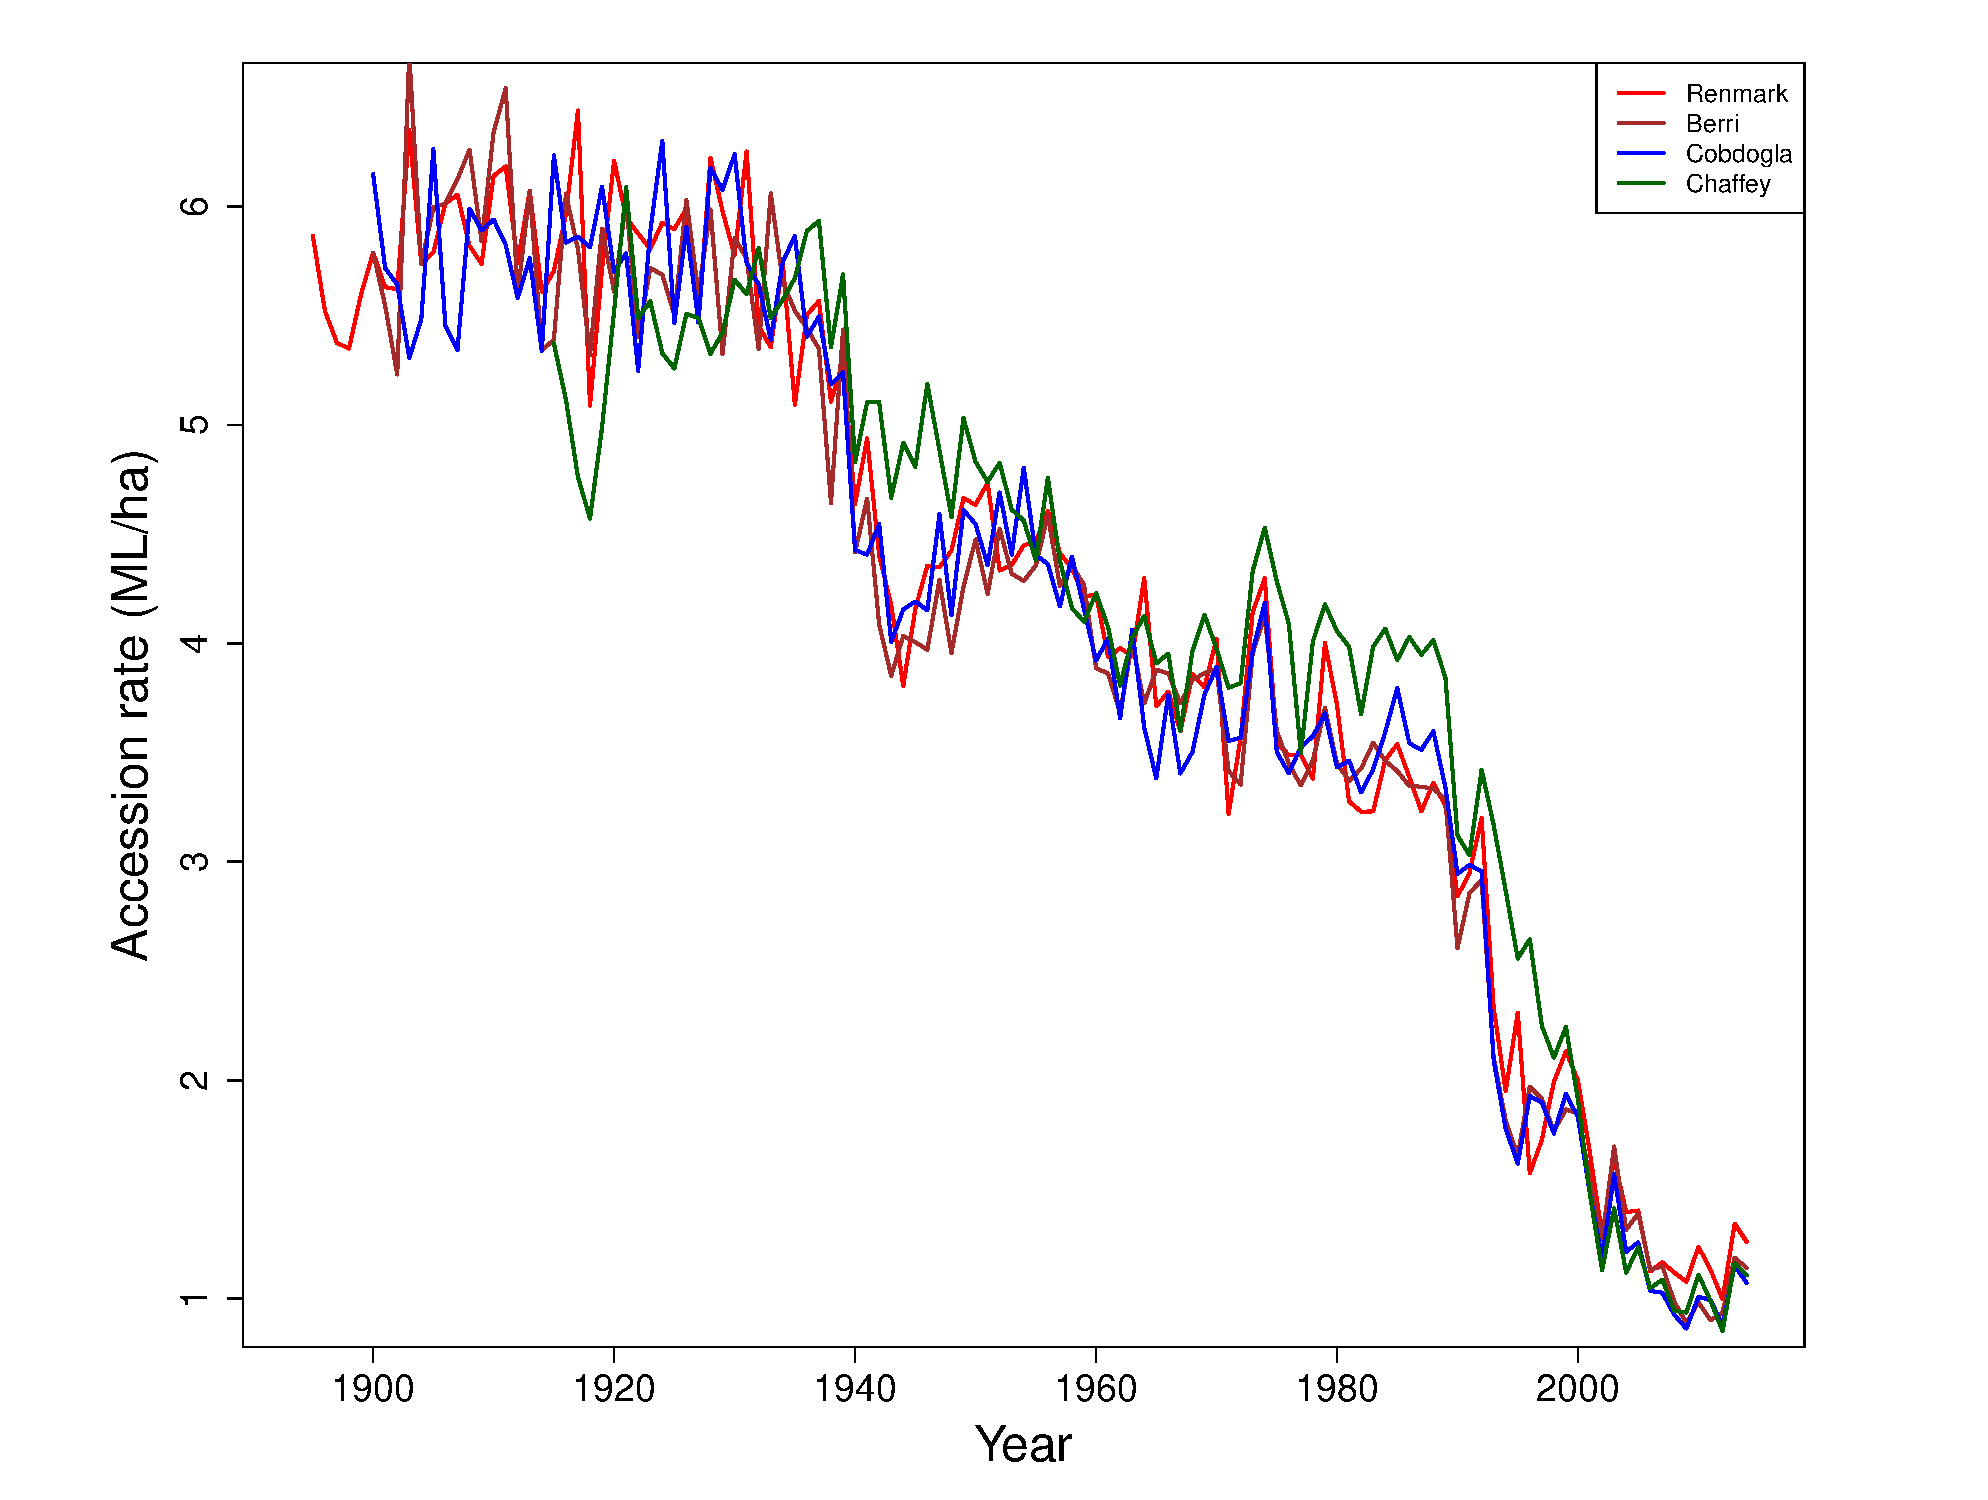
\includegraphics[width=0.95	extwidth]{../figures/plotacc-1} 

\end{knitrout}
\caption{Annual variation of irrigation accessions rate (ML/ha) for each of the irrigation districts of Cobdogla, Berri, Renmark and Chaffey from commencement of irrigation until 2014.}
\label{fig02}
\end{figure}


\subsection{Comments of Estimated Accession Volumes}
The irrigation accessions volumes are best estimates given the level of understanding of irrigation in the Riverland and was hampered by the quality and quantity of measured data of area, pumped volumes and application rates. It would be unwise to give an estimate of the error in the data before 1992.

An explanation of the important parameters determing irrigation accession can be found in the Lyrup, Simarloo, Pike and Murtho 2014 report of \citet{Meissner2014}.

\newpage
%\section{References}
\begin{thebibliography}{20}

\bibitem[Adams and Meissner(2009)]{Adams2009} Adams, A. and Meissner, T (2009) How Efficient are We. Report prepared for Department For Water by PIRSA Rural Solutions and Laroona Environmetrics, December 2009.

\bibitem[Dastane(1978)]{Dastane} Dastane, N.G. (1978) Effective Rainfall.  FAO Irrigation and Drainage Paper 25. M-56 ISBN 92-5-100272-X  \url{http://www.fao.org/docrep/X5560E/X5560E00.htm}

\bibitem[Meissner(2012)]{Meissner2012} Meissner, Tony 2012. Estimation of Accession Volumes of the Woolpunda Irrigation Areas. Report prepared for Department for Environment, Water and Natural Resources, Adelaide by Laroona Environmetrics, Loxton,  October 2012.

\bibitem[Meissner(2011a)]{Meissner2011a} Meissner, Tony (2011) Estimation of Accession Volumes of the Loxton and Bookpurnong Irrigations Areas. Report prepared for Department for Water by Laroona Environmetrics, Loxton, February 2011.

\bibitem[Meissner(2011b)]{Meissner2011b} Meissner, Tony (2011) Estimation of Accession Volumes of the Cadell, Qualco-Sunlands and Waikerie Irrigations Areas. Report prepared for Department for Water by Laroona Environmetrics, Loxton, November 2011.

\bibitem[Meissner(2014)]{Meissner2014} Meissner, Tony (2014) Estimation of Irrigation Accession Volumes for the Lyrup, Pike and Murtho Districts. Report to Department of Environment, Water and Natural Resources by Laroona Environmetrics, Loxton, August 2014.

\bibitem[Middlemis, Georgiou, and Richardson(2009)]{REM} Middlemis, H.,  Georgiou, J \& Richardson, S (2005) Pike River and Murtho Concept Design for Salt Interception Schemes, Groundwater Model.  Report prepared by Resource \& Environmental Management for the Department of Water Land and Biodiversity Conservation, August 2005

\end{thebibliography}

\newpage
\begin{appendices}
% graphs of irrigated area, application rate (ML/ha) and accession rates (ML/ha) for each
% of the irrigation areas

\section{Excel\textsuperscript{\textregistered} Spreadsheets} \label{excel} The template containing the district worksheets of calculations to estimate water draining beyond the rootzone is the file \textit{Irrigation Accessions.xlsx}. Also attached is the file \textit{rainfall.xlsx} containing the rainfall data.

\begin{sidewaysfigure}
\section{Cobdogla}
\begin{knitrout}
\definecolor{shadecolor}{rgb}{0.969, 0.969, 0.969}\color{fgcolor}
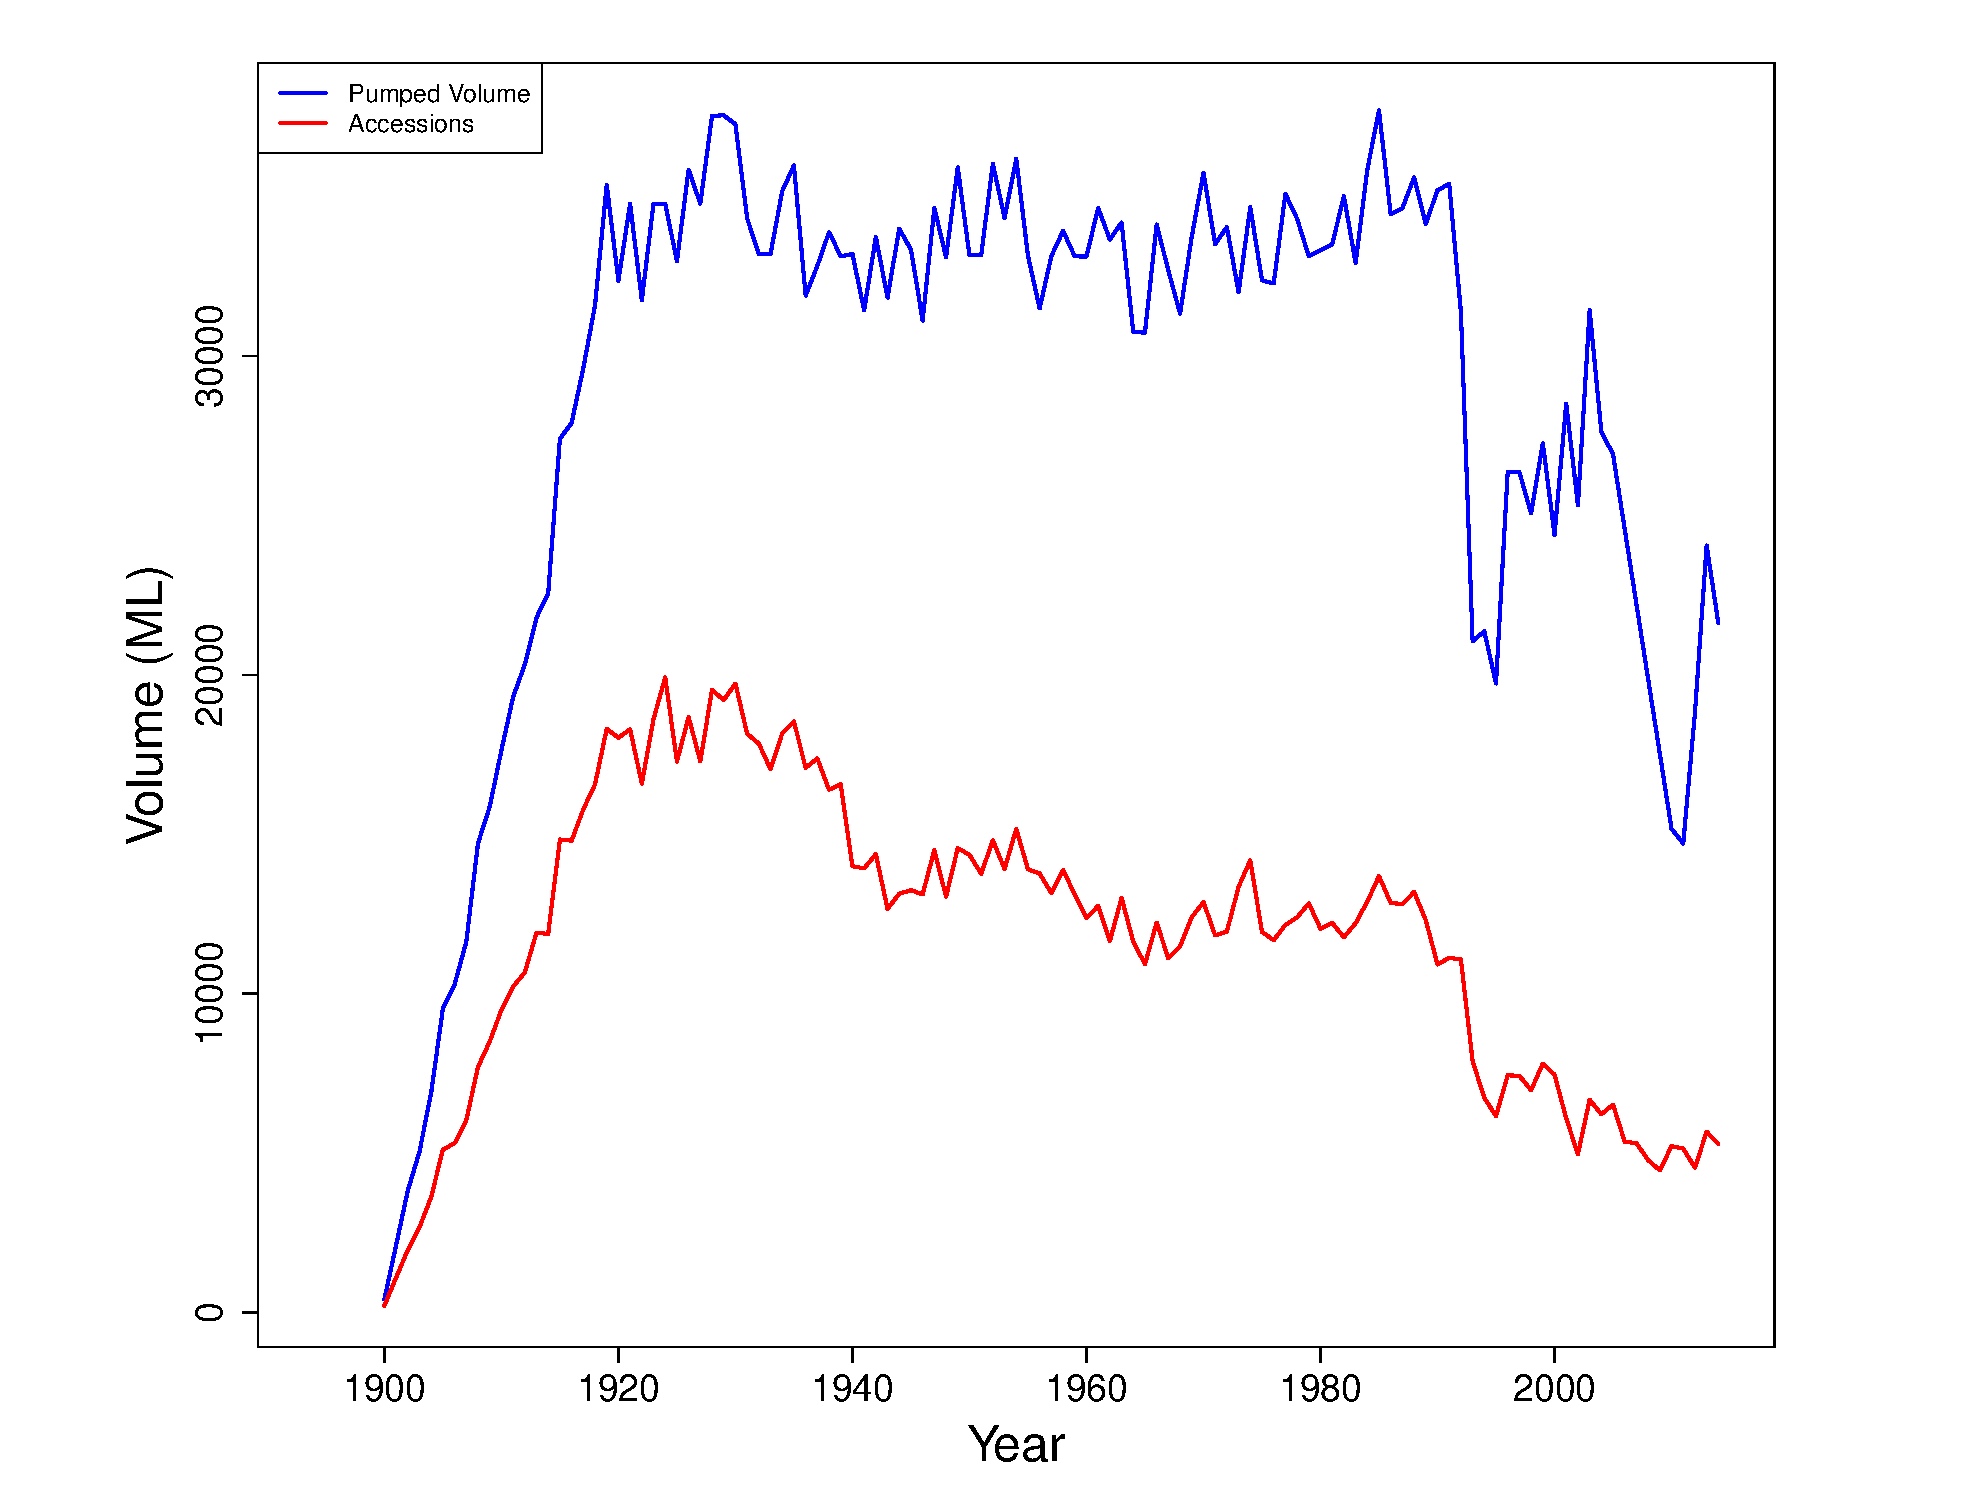
\includegraphics[width=0.95	extwidth]{../figures/Cobdogla-1} 

\end{knitrout}
\caption{Pumped irrigation and accession volumes for the Cobdogla Irrigation district 1900 -- 2014}
\label{fig03}
\end{sidewaysfigure}

# Berri 
\begin{sidewaysfigure}
\section{Berri}
\begin{knitrout}
\definecolor{shadecolor}{rgb}{0.969, 0.969, 0.969}\color{fgcolor}
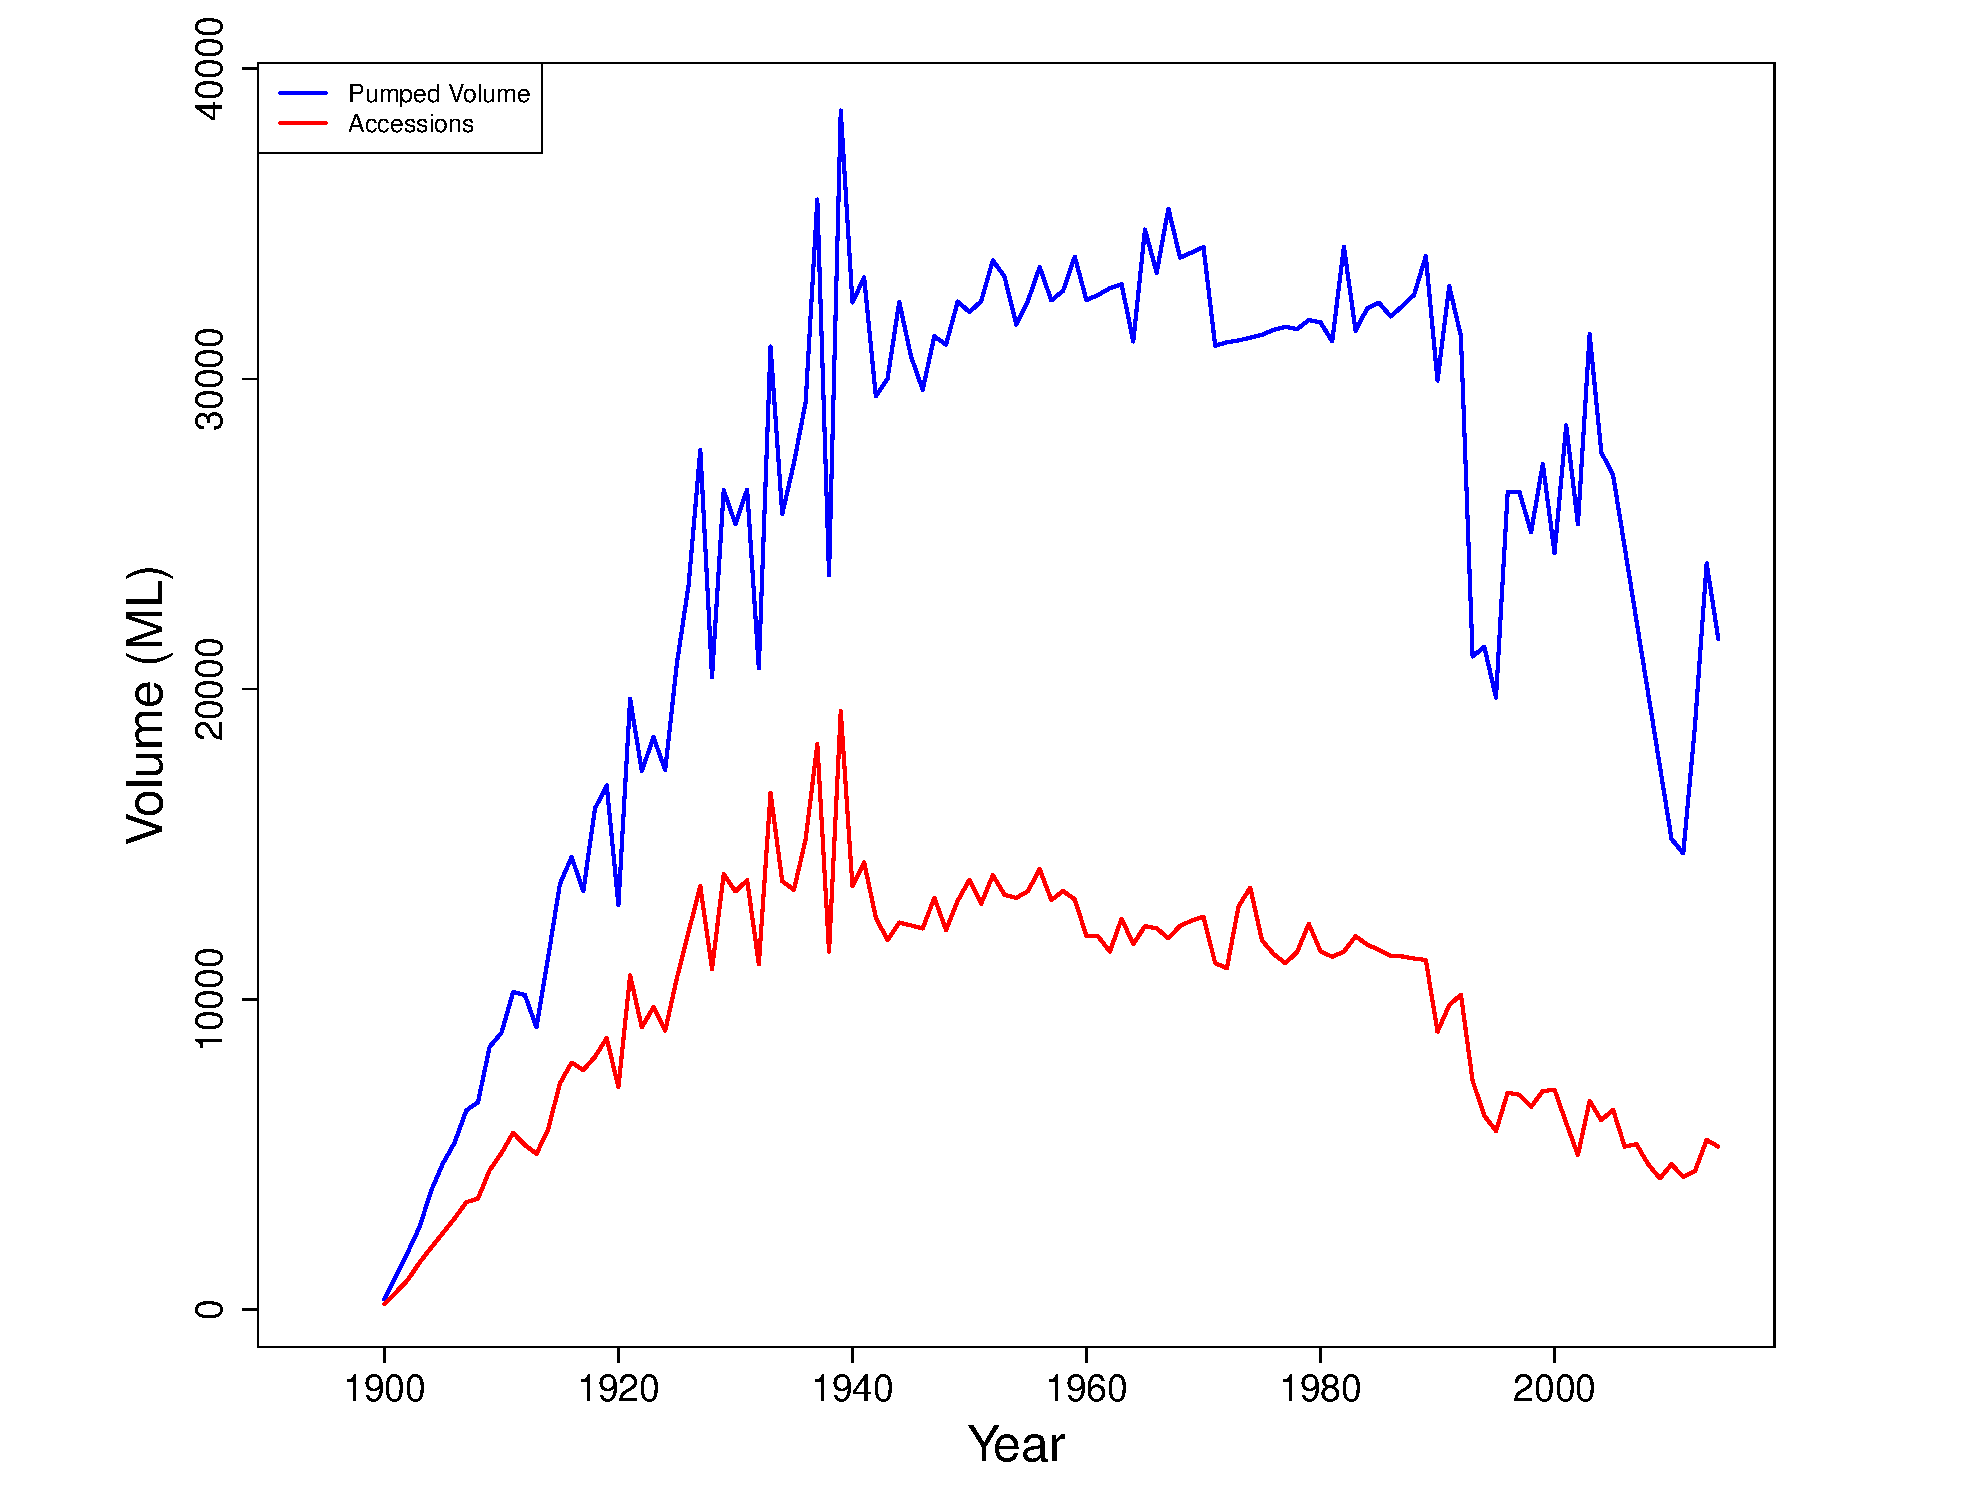
\includegraphics[width=0.95	extwidth]{../figures/Berri-1} 

\end{knitrout}
\caption{Pumped irrigation and accession volumes for the Berri Irrigation district 1900 -- 2014}
\label{fig03}
\end{sidewaysfigure}


# Renmark 
\begin{sidewaysfigure}
\section{Renmark}
\begin{knitrout}
\definecolor{shadecolor}{rgb}{0.969, 0.969, 0.969}\color{fgcolor}
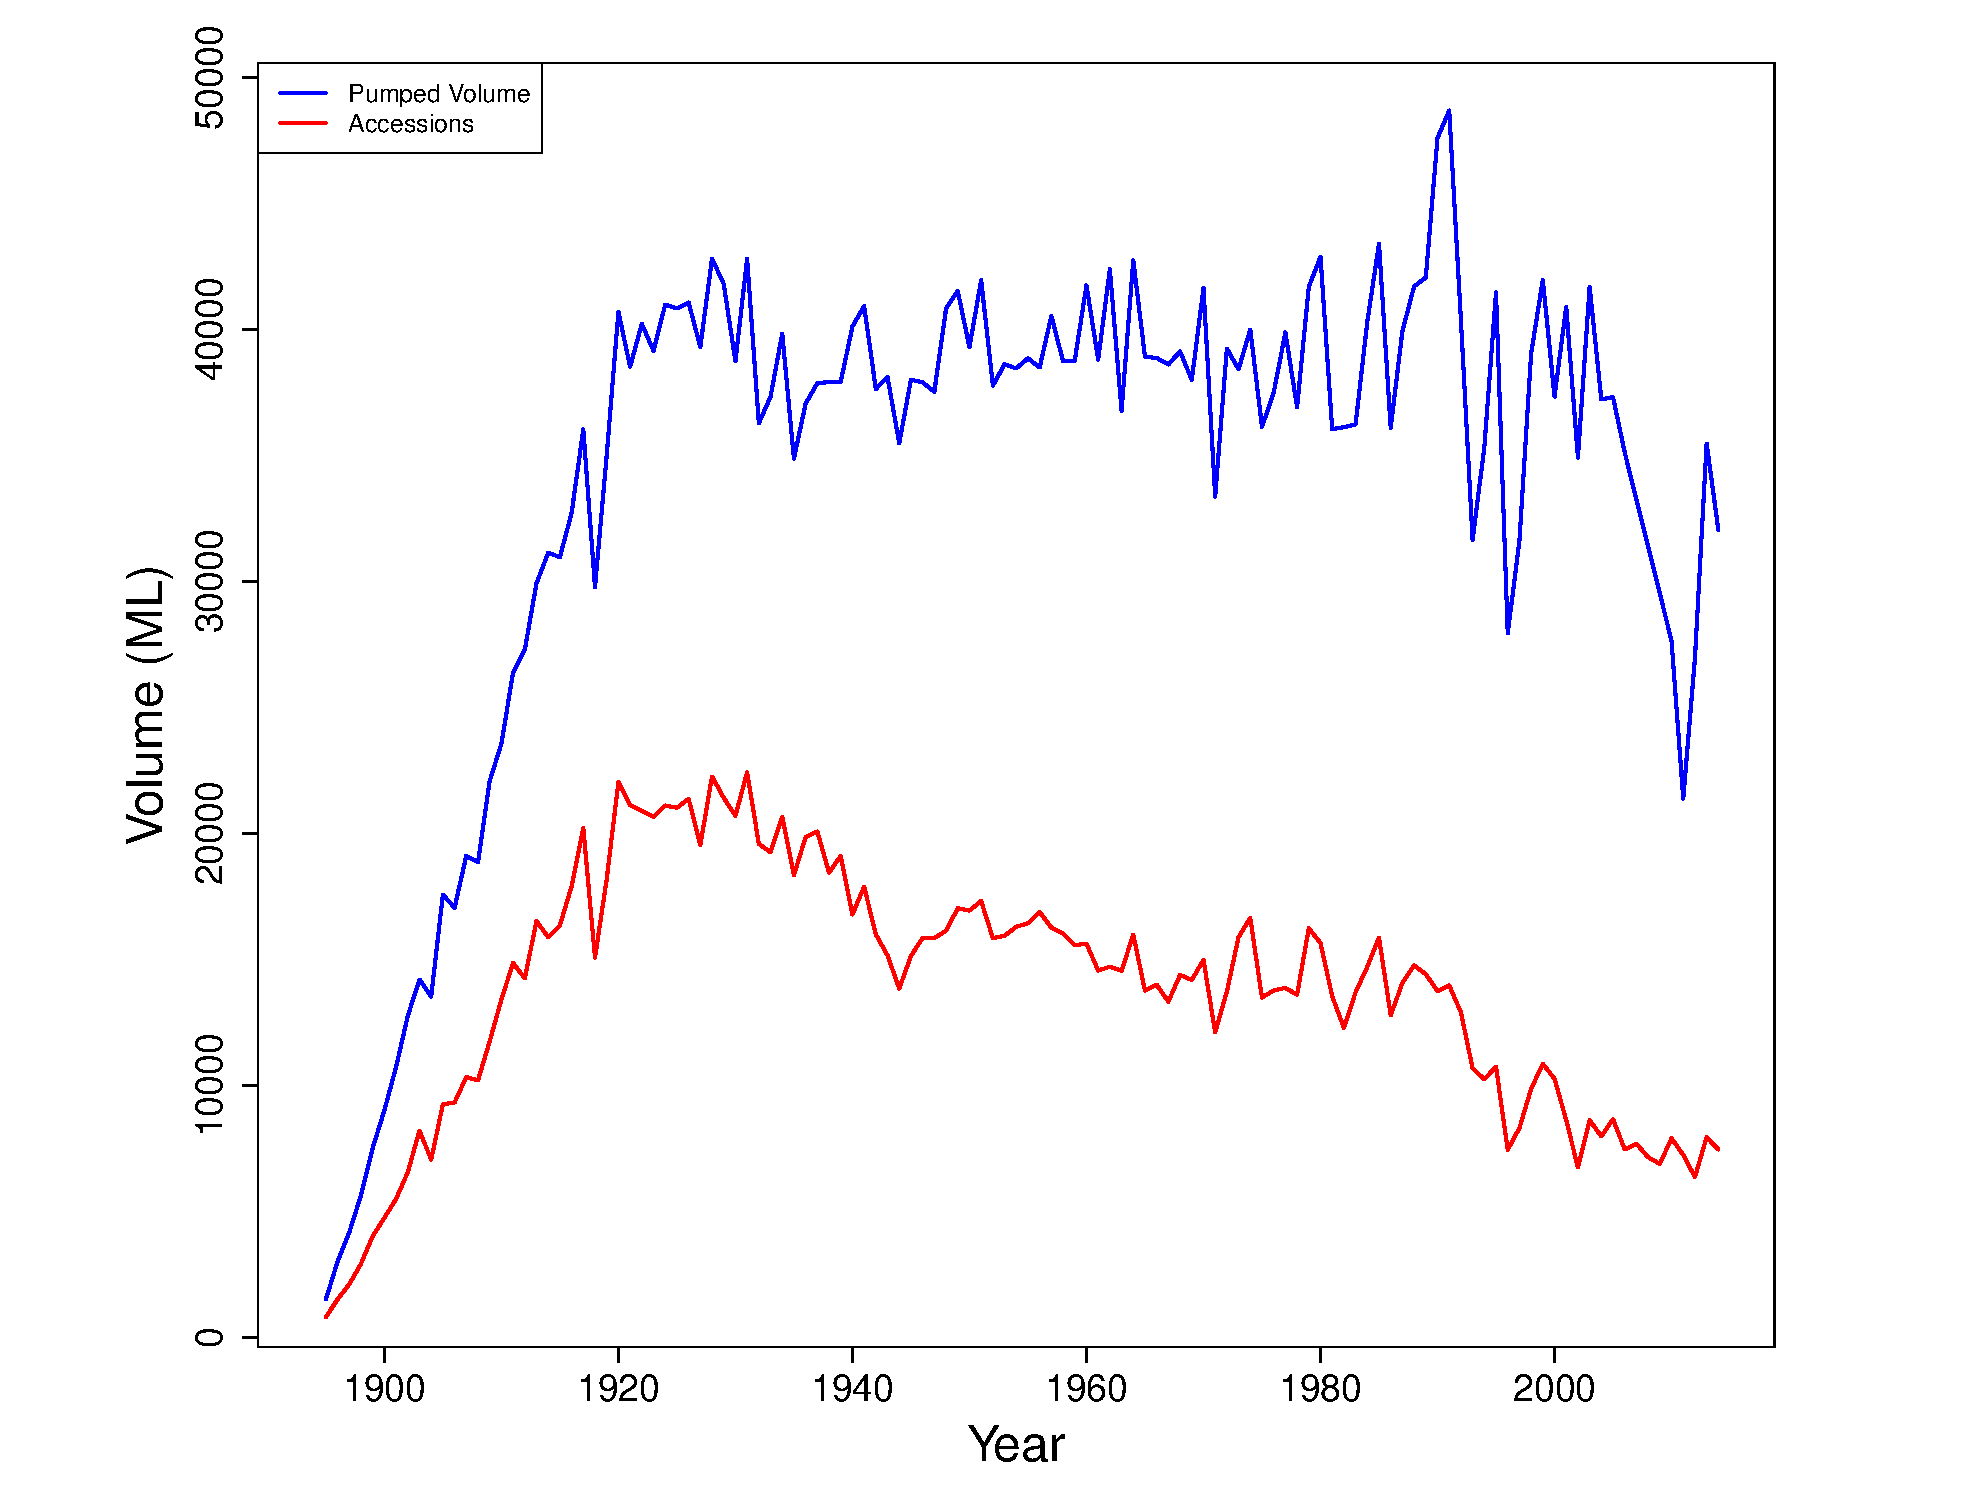
\includegraphics[width=0.95	extwidth]{../figures/Renmark-1} 

\end{knitrout}
\caption{Pumped irrigation and accession volumes for the Renmark Irrigation district 1900 -- 2014}
\label{fig03}
\end{sidewaysfigure}

# Chaffey 
\begin{sidewaysfigure}
\section{Chaffey}
\begin{knitrout}
\definecolor{shadecolor}{rgb}{0.969, 0.969, 0.969}\color{fgcolor}
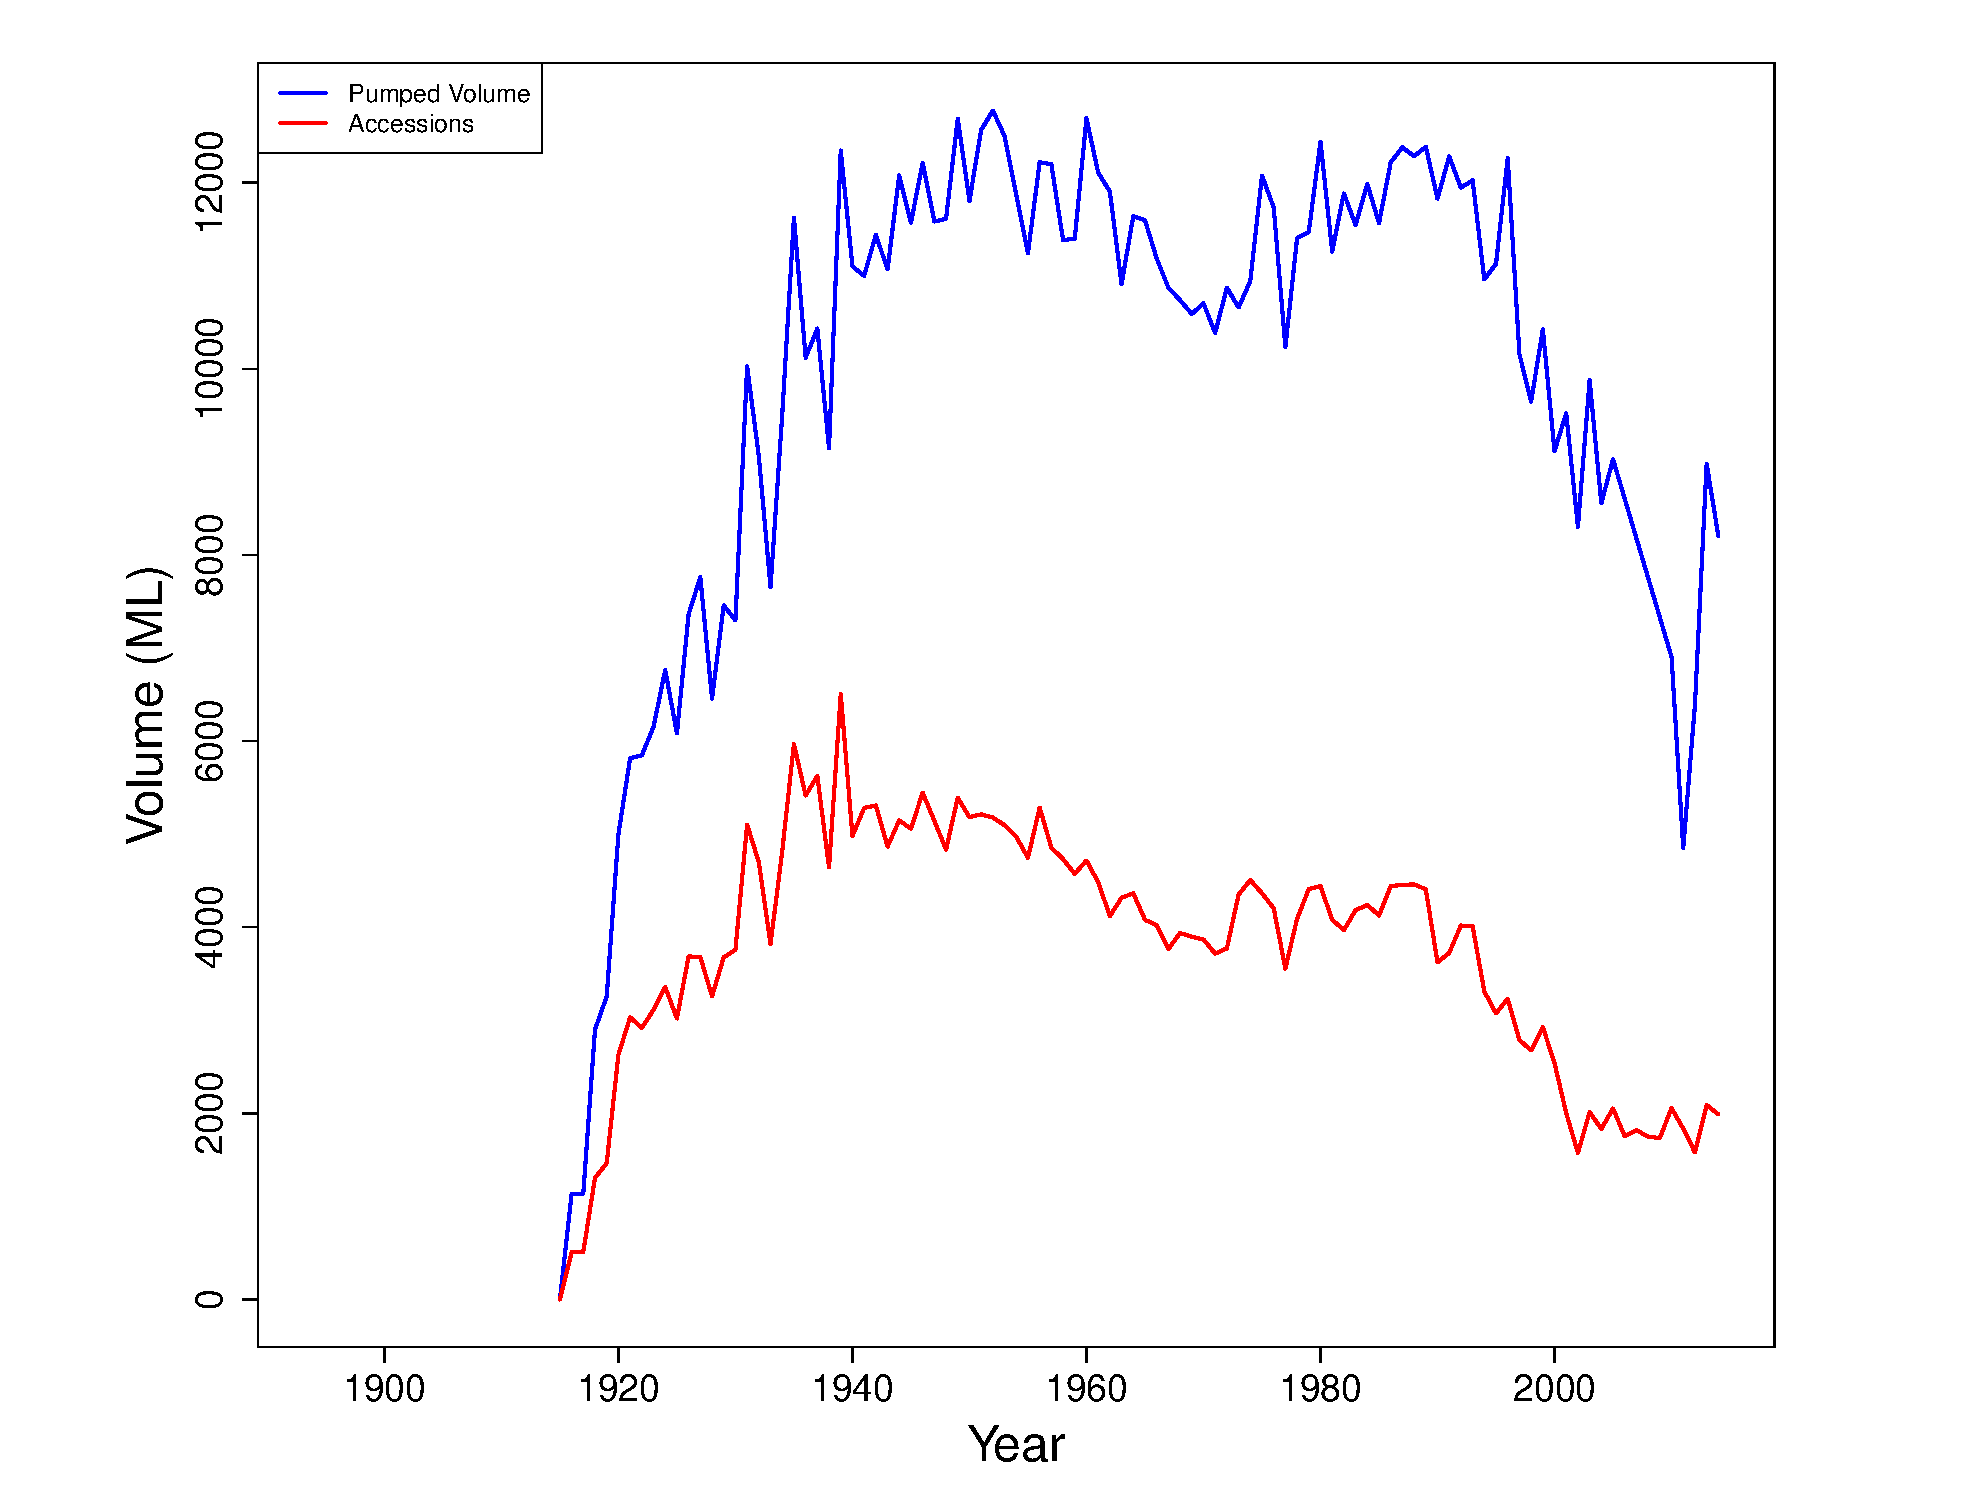
\includegraphics[width=0.95	extwidth]{../figures/Chaffey-1} 

\end{knitrout}
\caption{Pumped irrigation and accession volumes for the Chaffey Irrigation district 1900 -- 2014}
\label{fig03}
\end{sidewaysfigure}
\end{appendices}


\end{sffamily}
\end{document}
